In this section, basic approaches how to focus a laser beam in experiments are discussed. Before providing a brief overview of currently used methods, it is necessary to introduce several most fundamental parameters that describe any optical system. First, one defines a numerical aperture of an optical system $ N\!A $, which is a dimensionless number characterizing the range of angles over which the system can accept or emit light. Second characteristic of any optical system is a focal length $ f $ describing a distance between the center of the aperture and the point in space over which collimated light rays are brought to a focus. Finally, one defines a f-number $ f/\# $ as a ratio of the focal length $ f $ to the size of the aperture $ D $. The f-number $ f/\# $ is dimensionless and stands for a quantitative measure of a speed of the optical system.

In experiments, focusing of laser beams is usually achieved by means of an optical system, such as a lens or a curved mirror. However, when dealing with a short pulses, lenses are not preferred because they may affect the beam by frequency-dependent effects, such as chromatic aberration and other nonlinear optical distortions. On the other hand, reflective optics are generally able to produce a diffraction limited image without chromatic effects.

An off-axis parabolic (OAP) mirror is a frequently used tool to focus an incoming collimated beam. OAP is made by cutting out a small section from a full parabolic mirror and thus it allows to deviate the beam path off the optical axis. Therefore, the parts of incoming collimated beam do not overlap as in the case of a complete parabolic mirror and the focal point is at more accessible location. Obviously, OAP is able to work reversibly, so it can take the light coming from a point source and produce a collimated beam. These physical properties make OAP a valuable tool for many different optical purposes.

However, conventional solid state optic

%When using conventional solid state optics, these approaches typically require an increase in the beam diameter to keep the energy density on the optic below the damage threshold. Alternatively, the focal spot size can be decreased, by implementing a small F-number (F/#) focusing optic (large numerical aperture). Such optics are typically expensive and are susceptible to damage from target debris due to their short focal length (and thus close proximity to the target).

The development of single-use, disposable plasma-based optics enables many of these short-comings to be avoided. Crucially, plasma mirrors operate at a much higher energy density and are therefore more than an order of magnitude smaller than conventional solid state optics, and can thus be manufactured at much lower cost. Their disposable nature means that target debris is not an issue.

%the distance between the target and the focusing optics decreases with decreasing the f/#, so care must be taken to protect the mirror surface from debris induced by the exploded target flow after laser irradiation.

One way to alternate the concern of damage only the optics is to use plasma-based optics, there so called “plasma mirror (PM)” [2] were proposed and investigated in detail [3].Such plasma-based mirror is single-use, thus concerns about debris will naturally eliminated. In addition, as plasmas are already ionized, the PM can be used under much higher laser energy fluence than solid optics where fluence is restricted by their damage threshold (~1011 W/cm2), i.e. under at least 100-times higher fluence compare to the damage threshold of solid optics (typically 0.1-1 J.cm-2 for ~1ps laser pulse [4]). Thus, the optics size can be reduced by at least a factor of 10. Thus, the PM is more like laser experiment targets, rather than permanent mirrors. This change in thinking frees us from the anxiety of protecting the focusing optics from solid target debris after shots, thus enabling us to shorten dramatically the distance between the mirror surface and the target. In addition, a plasma mirror can enhance the temporal and spatial contrast ratio of the laser [5] [6] which improve the light pulse quality for many applications,

When an intense femtosecond pulse (I > 1016 W/cm2) hits an optically polished solid surface, it generates a dense plasma that itself acts as a mirror, known as a plasma mirror (PM).1 PMs do not just reflect the remainder of the incident beam, but can act as active optical elements that can be used for improving the temporal contrast of modern ultrahigh intensity lasers

the intensities stay below the damage threshold of these components.

but this comes at the risk of damaging the optics with target debris, as it requires their placement in close proximity to the interaction region.

The basic principle of the plasma mirror is that a thin plasma is created on the surface of a solid which is otherwise transparent to the laser light. Laser light is reflected at the critical density. In this way, the main pulse which is reflected from the plasma has a sharper rising edge and higher intensity contrast.

%The fact that light is reflected from a thin plasma layer formed on the substrate surface means that the surface can be curved to induce focusing (just as in conventional solid state optics). By appropriate choice of the surface curvature, an incident focusing laser beam can be made to focus with an even smaller F/#. A focusing plasma mirror (FPM) of ellipsoidal geometry with two foci, such that demagnification of a focal spot occurs from one focal position to the other, satisfies the need to have off-axis focusing to ensure that the target is not blocking the incoming laser beam. Such an optic is attractive not only because of the increase in peak laser intensity achievable but also because it improves pulse intensity contrast in the same way as a PPM.

In practical terms, a conventional OAP can be aligned such that the focus coincides with f1 of the FPM. As the light diverges beyond f1, it reflects from the plasma it forms on the curved optic surface and is imaged to position f2. The focal spot at f1 is demagnified at f2 depending on the chosen geometry of the FPM and the angle hin.

The common approach to focusing an intense laser beam is to use a large laser beam size with conventional optical components, such as mirrors and lenses, so that the intensities stay below the damage threshold of these components. This approach imposes limits upon the geometrical characteristics of the focused beam such as the focal spot size and focal length

As soon as intensities reach 1013W/cm2, any medium becomes strongly ionized by the field, making conventional optics inappropriate in this regime, and thus optical components will inevitably consist of a plasma medium.

When a pulse from such a laser hits an optically polished surface, it generates a dense plasma that itself acts as a mirror, known as a plasma mirror (PM). PMs do not just reflect the remainder of the incident beam, but can act as active optical elements.

consists of reflecting the laser beam on a dielectric target with an initially low reflectivity. The target reflectivity strongly increases when this plasma becomes dense enough to screen the incident laser field

can withstand higher laser intensities than conventional optics

to enhance the temporal contrast.

An ellipsoidal, focusing PM configuration has also been shown, in principle, to be a capable replacement of the final focusing optic in the laser system

serve as a sacrificial last optical surface in hostile environments, which protects the expensive final focusing optic

Plasma devices are an attractive, compact alternative to tightly focus extreme light pulses and further increase the final laser intensity.

plasma mirrors not only focus laser pulses in space, but can also compress them in time.

%The typical optic aperture of ∼1 cm for the plasma focusing optic converts standard focusing of ultra-high intensity lasers to an extremely small f-number (e.g., f/#∼0.5). This optic simultaneously achieves: (1) tight focusing concomitant with a field intensity enhancement, and (2) enhancement of the temporal contrast of the laser, a parameter that is absolutely crucial for solid-interaction applications, such as the generation of high-order harmonics, directed electron beams, relativistic ions, etc. Currently, extremely small f/# conventional focusing optics for laser-solid interactions are not readily employable due to the high risk of damage to the optic due to the projection of target debris since the target has to be located close to the optic surface. Because an optic made of plasma is already in an ionized state, it is impervious to such damage, and thus can lead to extreme compacification of the optic. The ideal shape of such a plasma optic is an ellipsoid since it possesses no spherical aberration.

proposed using a short plasma channel as a focusing lens for laser pulses. Such a plasma lens would be able to tolerate laser intensities far above the usual damage limits for conventional optics. This offers the possibility of efficiently manipulating intense laser pulses whose spot size in the lens is far smaller than possible with conventional optics. Thus, it may substantially reduce the size of the overall system and allow the laser pulse to be manipulated very close to the interaction region. As long as the laser power is below the critical power for relativistic guiding, the focal length will be independent of the laser power within the pulse, and the plasma lens will focus the laser pulse in a manner similar to a conventional short focal length lens. The plasma lens may, in principle, be tuned by controlling the plasma density, making it possible to move the position of the focus without physically moving any optical component. If the plasma density has an on-axis minimum, it will behave as a positive or focusing lens.

offers versatility in the plasma lens small f-number for extremely tight focusing of high power lasers with no damage threshold restrictions of regular optical components

In the relativistic regime, curved PMs have been proposed as a way to focus the very high generated harmonic orders to a spot size smaller than the laser wavelength

Small size high precision optics could be mass-produced and replaced after each shot

It should be noted that the plasma optic has to be refreshed after each shot.

As the interaction zone is destroyed after every laser shot, the target surface must therefore be refreshed at the laser repetition rate while maintaining identical interaction conditions from shot to shot

Lens, off-axis parabola mirror - conventional solid state optic
ellipsoid plasma mirrors, plasma lens



\floatsetup[figure]{style=plain, subcapbesideposition=top}
\begin{figure}[h!]
	\centering
	\sidesubfloat[]{{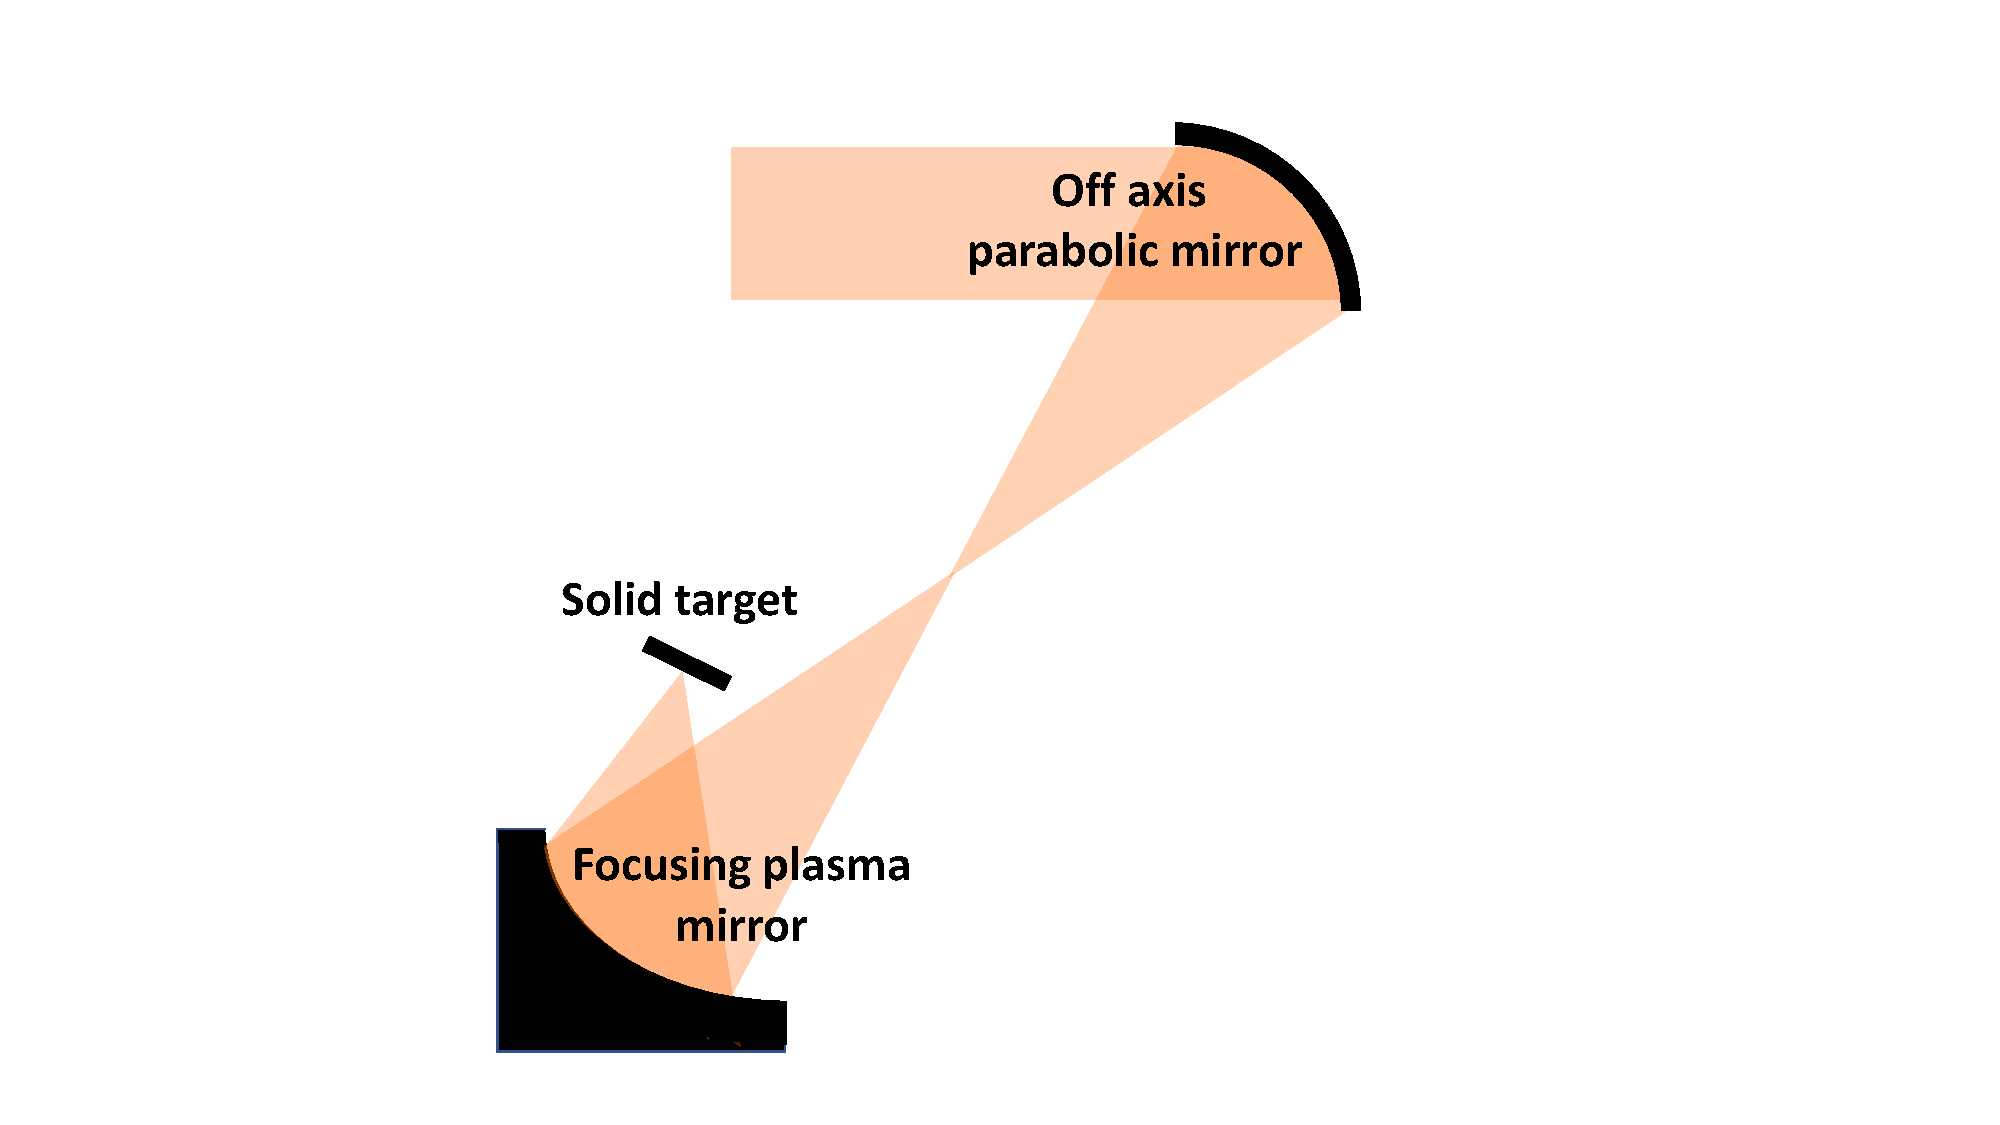
\includegraphics[width=0.35\linewidth]{./img/exp/diagram.pdf}}}
	\hspace{5mm}
	\sidesubfloat[]{{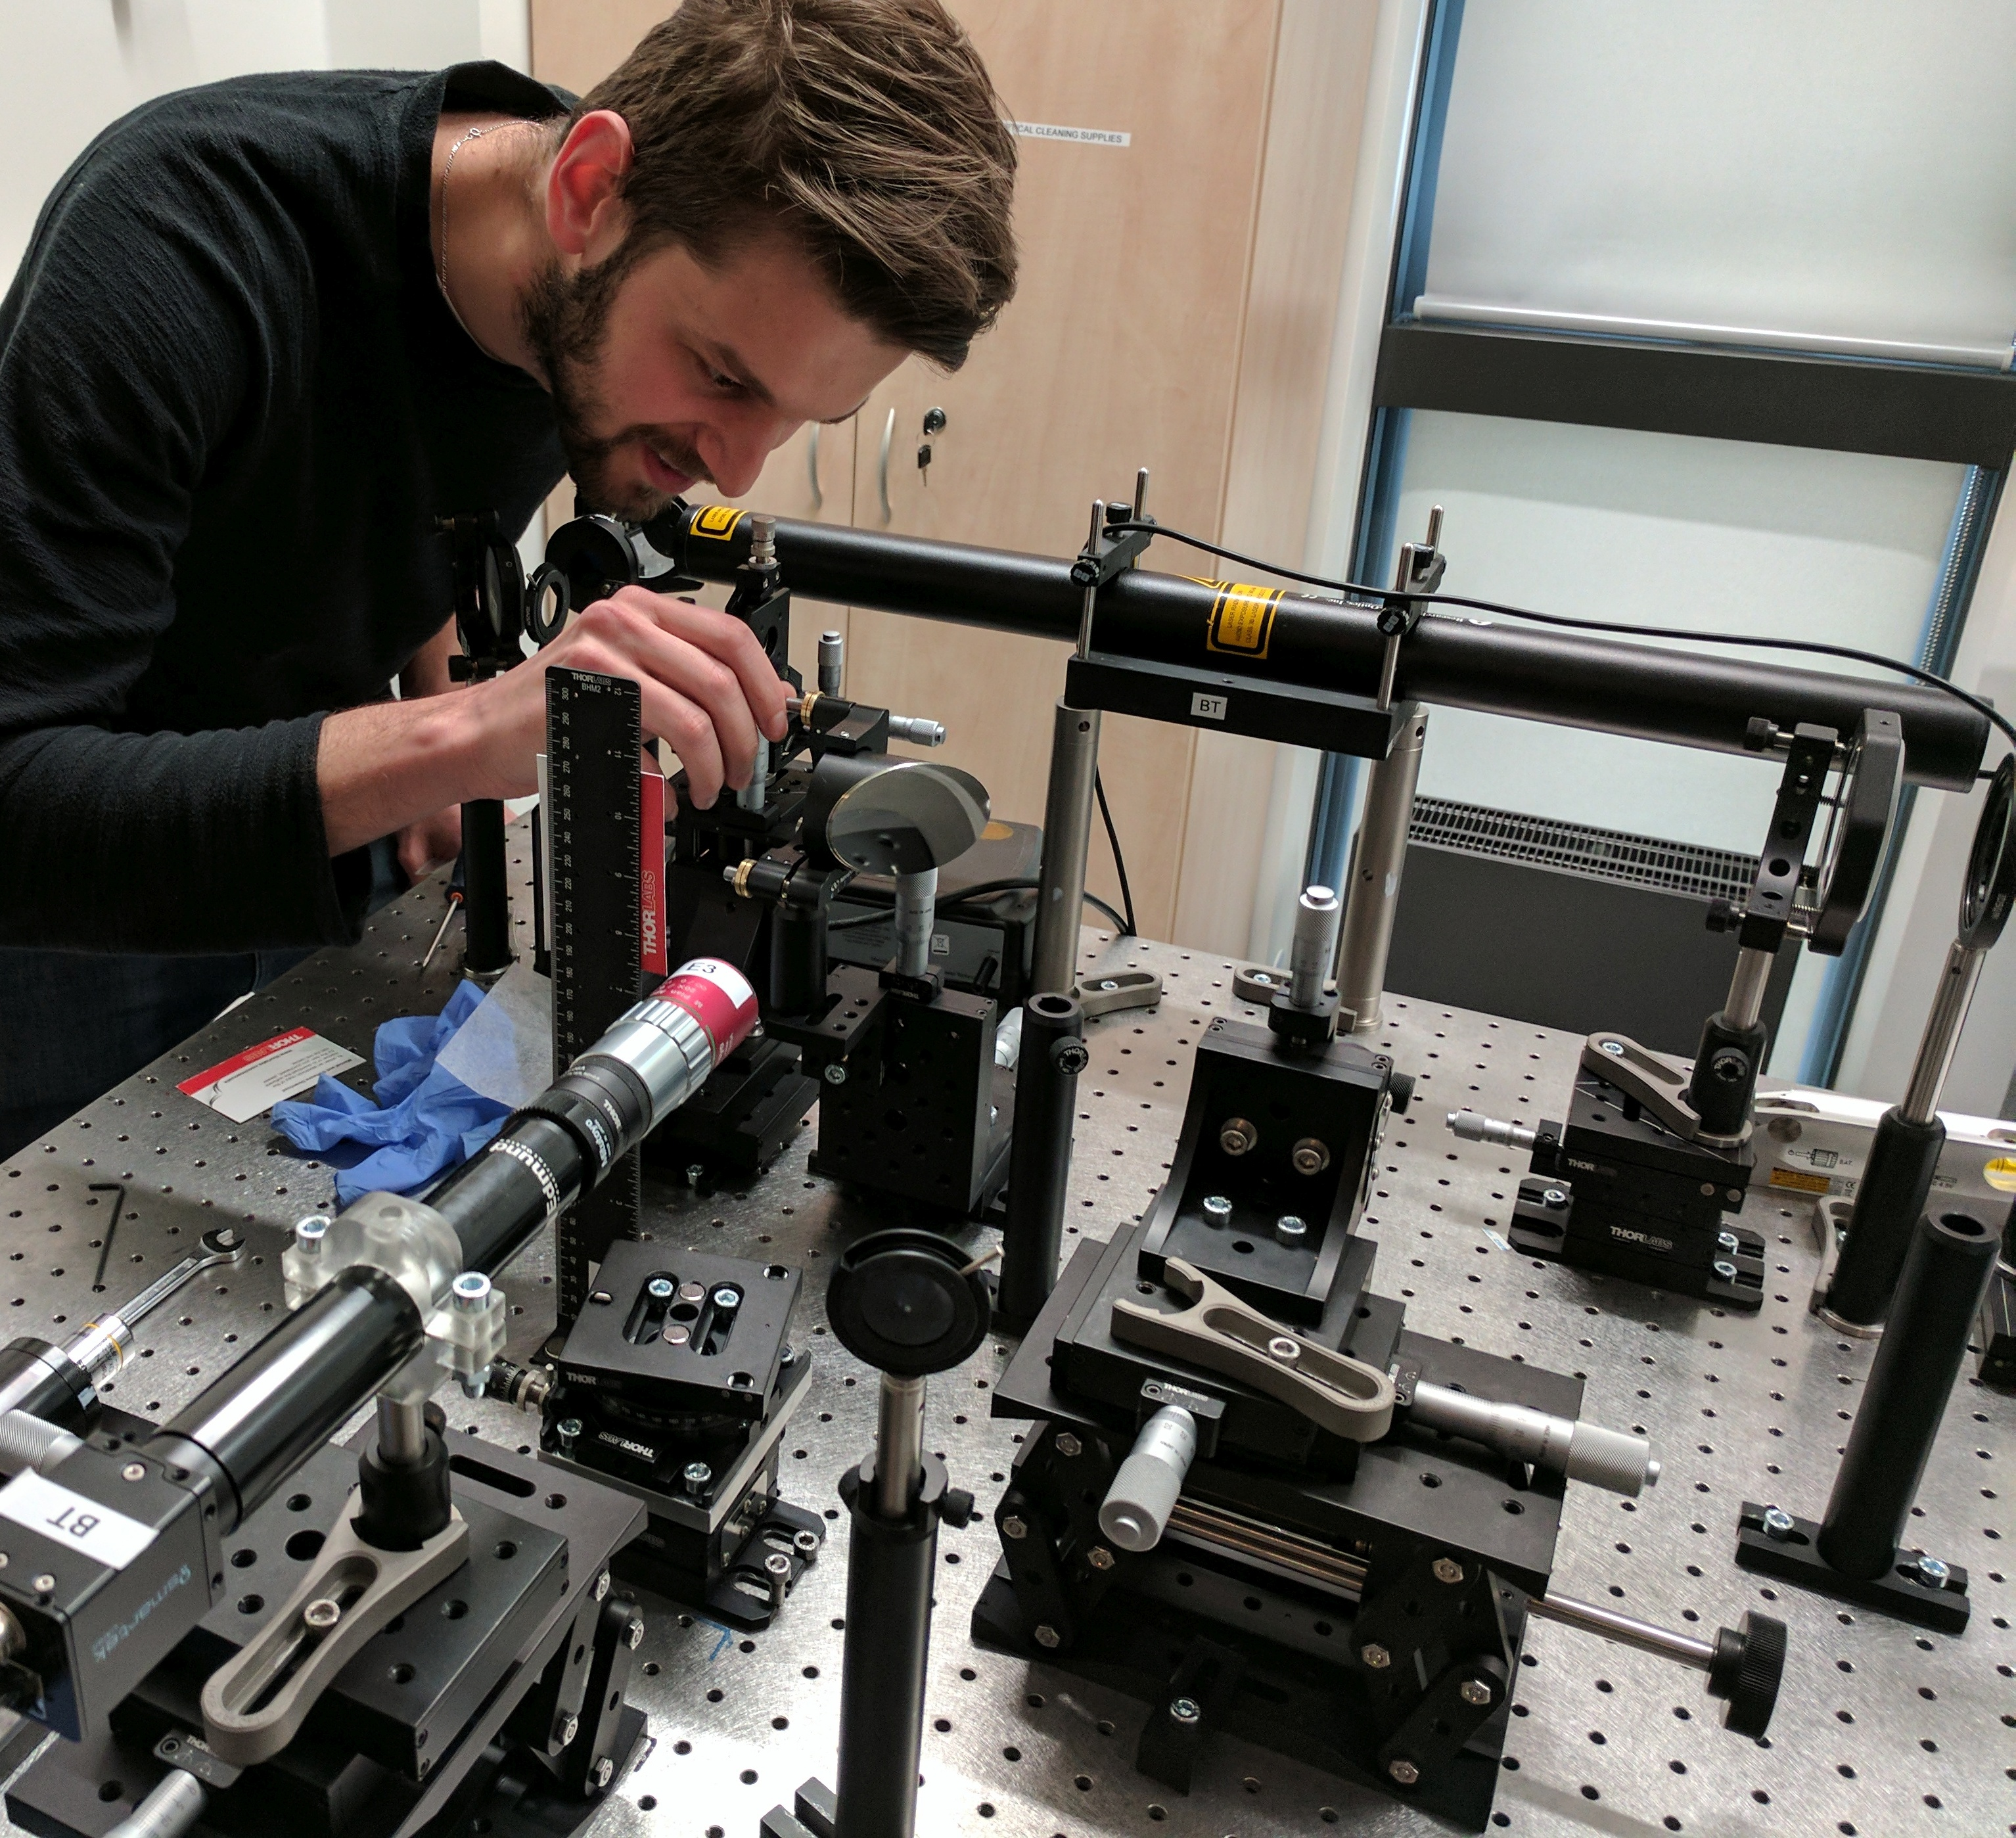
\includegraphics[width=0.4\linewidth]{./img/exp/photo2.jpg}}}
	\caption{\textbf{(a)} Schematic diagram showing the operation of the focusing plasma mirror where the incoming laser beam is focused by a conventional off-axis parabolic mirror. The plasma mirror focuses the beam onto a target surface. \textbf{(b)} Photo capturing a very long and frustrating process of aligning an off-axis parabolic mirror.}
	\label{}
\end{figure}